\section{Power-scale corrections and exponential mass concentration}
\label{rwbound:real:sec:boundary}

The atom in Theorem~\ref{subunit:thm:domain} raises a quantitative
question: how does an absolutely continuous positive part collapse into
that atom? Two distinct scales occur. Its outermost point approaches the
endpoint by a power of the distance to the critical line. Most of its
mass lies much closer to the endpoint, on an exponential scale described
by a limiting exponential distribution.

Fix $b\in(0,1)$, and write
\begin{equation}\label{rwbound:real:eq:boundary-parameters}
 p=1-b,\qquad a=p+\varepsilon,\qquad
 K_\varepsilon(T)=K_{p+\varepsilon,b}(T),\qquad
 0<\varepsilon\leq\varepsilon_0<b.
\end{equation}
Let $T_\varepsilon$ be the unique logarithmic crossing of
$K_\varepsilon$, so $K_\varepsilon>0$ on $(0,T_\varepsilon)$.
All constants below may depend on the fixed $b$; the local expansion
constants may also depend on its chosen radius $T_0$.

\begin{lemma}[A uniform local kernel expansion]
\label{rwbound:real:lem:boundary-expansion}
For any fixed $T_0<2\pi$, uniformly for
$0\leq\varepsilon\leq\varepsilon_0$ and $0<T\leq T_0$,
\begin{equation}\label{rwbound:real:eq:boundary-expansion}
\begin{split}
 K_\varepsilon(T)=T^{\varepsilon-1}\biggl\{
 &\frac{\varepsilon}{p\Gamma(1+\varepsilon)}
 +\frac{\zeta(b)}{\Gamma(p+\varepsilon)}T^p
 -\frac{T}{2\Gamma(1+\varepsilon)}\\
 &-\frac{bT^2}{12\Gamma(2+\varepsilon)}+O_{b,T_0}(T^4)
 \biggr\}.
\end{split}
\end{equation}
More generally the bracket has the convergent expansion
\begin{equation}\label{rwbound:real:eq:boundary-series}
\begin{split}
 &\frac{\varepsilon}{p\Gamma(1+\varepsilon)}
 +\frac{\zeta(b)}{\Gamma(p+\varepsilon)}T^p
 -\frac{T}{2\Gamma(1+\varepsilon)}\\
 &\hspace{8mm}
 -\sum_{\ell\geq1}\frac{B_{2\ell}\Gamma(b+2\ell-1)}
 {(2\ell)!\,\Gamma(b)\Gamma(\varepsilon+2\ell)}T^{2\ell},
 \qquad 0<T<2\pi.
\end{split}
\end{equation}
Here $B_{2\ell}$ are the Bernoulli numbers, with $B_2=1/6$.
\end{lemma}

\begin{proof}
In \eqref{subunit:eq:generalK}, put $a=p+\varepsilon$ and
$a+b=1+\varepsilon$. The common regularizer has the convergent expansion
\[
 q(t)=\frac12+\sum_{\ell\ge1}\frac{B_{2\ell}}{(2\ell)!}t^{2\ell-1},
 \qquad |t|<2\pi.
\]
Its positive convolution therefore has expansion
\[
 C_{a,b}(T)=\frac{T^\varepsilon}{2\Gamma(1+\varepsilon)}
 +\sum_{\ell\ge1}\frac{B_{2\ell}\Gamma(b+2\ell-1)}
 {(2\ell)!\Gamma(b)\Gamma(\varepsilon+2\ell)}T^{\varepsilon+2\ell-1}.
\]
The beta integral evaluates each coefficient. Substitute this into
\eqref{subunit:eq:generalK} and use
$\Gamma(1+\varepsilon)=\varepsilon\Gamma(\varepsilon)$ to obtain
\eqref{rwbound:real:eq:boundary-series}. For uniform remainders choose
$T_0<T_1<2\pi$; Cauchy estimates bound the regularizer's Taylor remainder
on $|t|\le T_0$, while $v^{b-1}(1-v)^{p-1}$ dominates all beta weights.
The Gamma factors are bounded on the fixed compact parameter interval.
This proves the uniform truncation and the full locally convergent series.
\end{proof}

\begin{theorem}[Crossing scale and its first correction]
\label{rwbound:real:thm:boundary-crossing}
Define
\begin{equation}\label{rwbound:real:eq:tau}
 \tau_\varepsilon=
 \left\{\frac{\Gamma(p+\varepsilon)\varepsilon}
 {p[-\zeta(b)]\Gamma(1+\varepsilon)}\right\}^{1/p}.
\end{equation}
As $\varepsilon\downarrow0$,
\begin{equation}\label{rwbound:real:eq:crossing-correction}
 T_\varepsilon
 =\tau_\varepsilon-\frac{\tau_\varepsilon^2}{2\varepsilon}
   +O_b\!\left(\frac{\tau_\varepsilon^3}{\varepsilon^2}\right).
\end{equation}
In particular, with
\begin{equation}\label{rwbound:real:eq:boundary-constant}
 K_b=\left\{\frac{\Gamma(1-b)}{(1-b)[-\zeta(b)]}\right\}^{1/(1-b)},
\end{equation}
one has
\begin{equation}\label{rwbound:real:eq:crossing-leading}
 T_\varepsilon\sim K_b\varepsilon^{1/(1-b)},\qquad
 1-r_{p+\varepsilon,b}\sim K_b\varepsilon^{1/(1-b)}.
\end{equation}
\end{theorem}

\begin{proof}
For every fixed $T>0$, the kernel depends continuously on
$\varepsilon$ and its limit $K_{p,b}(T)$ is strictly negative by
\eqref{subunit:eq:criticaldensity}. The unique crossing therefore
satisfies $T_\varepsilon\to0$. At that crossing, multiply the
bracket in \eqref{rwbound:real:eq:boundary-expansion} by
$\Gamma(1+\varepsilon)$ and write
\[
 C_\varepsilon=
 \frac{[-\zeta(b)]\Gamma(1+\varepsilon)}{\Gamma(p+\varepsilon)}>0.
\]
This gives
\begin{equation}\label{rwbound:real:eq:crossing-equation}
 \frac{\varepsilon}{p}
 =C_\varepsilon T_\varepsilon^p+
   \frac{T_\varepsilon}{2}
   +\frac{bT_\varepsilon^2}{12(1+\varepsilon)}
   +O_b(T_\varepsilon^4).
\end{equation}
Since $p<1$, the last three terms are lower order than
$T_\varepsilon^p$. Hence
$T_\varepsilon/\tau_\varepsilon\to1$.

Put $y=T_\varepsilon/\tau_\varepsilon$ and
$q=\tau_\varepsilon/\varepsilon$.
The leading equivalence implies $q=O_b(\varepsilon^{b/p})\to0$.
Dividing \eqref{rwbound:real:eq:crossing-equation} by $\varepsilon/p$
gives, uniformly for $y$ near one,
\[
 1=y^p+\frac p2 qy+O_b(\varepsilon q^2).
\]
The mean value theorem first yields $y-1=O_b(q)$. Taylor expansion
then yields $p(y-1)+(p/2)q=O_b(q^2)$, so
$y=1-q/2+O_b(q^2)$. This proves
\eqref{rwbound:real:eq:crossing-correction}. Formula
\eqref{rwbound:real:eq:crossing-leading} follows from continuity of the
gamma factors and $1-e^{-T}\sim T$.
\end{proof}

At the symmetric boundary point $b=p=1/2$, the analytic correction
from the gamma quotient and the nonlinear root correction have the
same relative order. Using $\psi(1/2)=-\gamma-2\log2$ gives the
explicit consequence
\begin{equation}\label{rwbound:real:eq:half-boundary}
\begin{split}
 T_\varepsilon={}&\frac{4\pi}{\zeta(1/2)^2}\varepsilon^2
 \left[1-
 \left(4\log2+\frac{2\pi}{\zeta(1/2)^2}\right)\varepsilon
 +O(\varepsilon^2)\right].
\end{split}
\end{equation}
For other $b$, retaining the exact gamma quotient in
$\tau_\varepsilon$ keeps the algebraic and fractional-power
corrections in \eqref{rwbound:real:eq:crossing-correction} unambiguous.

\begin{theorem}[Condensation and the exponential positive-mass law]
\label{rwbound:real:thm:boundary-mass}
Let $\nu_\varepsilon=\nu_{p+\varepsilon,b}$, and denote its positive
and negative parts by $\nu_\varepsilon^+$ and
$\nu_\varepsilon^-$, so $\nu_\varepsilon=
\nu_\varepsilon^+-\nu_\varepsilon^-$. Then
\begin{equation}\label{rwbound:real:eq:boundary-measures}
 \nu_\varepsilon^-\longrightarrow
       -\kappa_{p,b}(u)\,du\quad\hbox{in total variation},\qquad
 \nu_\varepsilon^+\Longrightarrow\frac1p\delta_1.
\end{equation}
In particular $\nu_\varepsilon\Longrightarrow\nu_{p,b}$.

Let $\lambda_\varepsilon$ be the pushforward of the finite positive
measure $p\,K_\varepsilon(T)^+e^{-T}\,dT$ under
$Y_\varepsilon=-\varepsilon\log T$. For all sufficiently small
$\varepsilon$ it is supported in $[0,\infty)$ and
\begin{equation}\label{rwbound:real:eq:exponential-law}
 \left\|\lambda_\varepsilon-e^{-y}\mathbf1_{y>0}\,dy
       \right\|_{\rm TV}
 =O_b\!\left(\varepsilon|\log\varepsilon|\right).
\end{equation}
The same convergence and rate hold after normalizing
$\lambda_\varepsilon$ to a probability measure.
\end{theorem}

\begin{proof}
For $T\leq T_0<1$, Lemma~\ref{rwbound:real:lem:boundary-expansion} gives
\begin{equation}\label{rwbound:real:eq:boundary-leading-density}
 K_\varepsilon(T)=
 \frac{\varepsilon}{p\Gamma(1+\varepsilon)}T^{\varepsilon-1}
       +R_\varepsilon(T),\qquad
 |R_\varepsilon(T)|\leq C_bT^{p+\varepsilon-1}.
\end{equation}
The first term is positive, so the negative part is bounded by
$C_bT^{p-1}$, an integrable bound independent of $\varepsilon$.
For $T\geq T_0$, formula~\eqref{subunit:eq:generalK} and
$0<C_{a,b}(T)<k_{a+b}(T)$ give a common polynomial majorant as
$a$ ranges over $[p,p+\varepsilon_0]$; hence
$e^{-T}|K_\varepsilon(T)|\leq
C_be^{-T}(1+T^{\varepsilon_0})$. Pointwise convergence and dominated
convergence prove the negative-part assertion in
\eqref{rwbound:real:eq:boundary-measures}. Its limiting mass is $1/p$ by
Theorem~\ref{subunit:thm:domain}. Each $\nu_\varepsilon$ has total
mass zero, so the positive masses have the same limit. Their supports
lie in $(e^{-T_\varepsilon},1)$, which shrinks to $1$; this proves
the positive weak limit.

For the quantitative distributional statement set
$y_\varepsilon=-\varepsilon\log T_\varepsilon$.
Theorem~\ref{rwbound:real:thm:boundary-crossing} gives
$y_\varepsilon=O_b(\varepsilon|\log\varepsilon|)$ and
$y_\varepsilon>0$ for small $\varepsilon$.
On the positive support $0<T<T_\varepsilon$, replace the density
in \eqref{rwbound:real:eq:boundary-leading-density} by its leading term
and replace $e^{-T}$ by one. The total variation error is at most
\[
 C_bT_\varepsilon^{p+\varepsilon}
     +C_b\varepsilon T_\varepsilon^{1+\varepsilon}
 =O_b(\varepsilon),
\]
because $T_\varepsilon^p=O_b(\varepsilon)$.
Total variation cannot increase under pushforward. With
$T=e^{-y/\varepsilon}$, the pushforward of the resulting leading
measure is exactly
\[
 \frac{e^{-y}}{\Gamma(1+\varepsilon)}
          \mathbf1_{y>y_\varepsilon}\,dy.
\]
Its total variation difference from the unit exponential density
is at most
$O(\varepsilon)+\int_0^{y_\varepsilon}e^{-y}\,dy$.
This proves \eqref{rwbound:real:eq:exponential-law}. Its mass consequently
differs from one by the same order; normalizing changes the total
variation by at most that mass discrepancy.
\end{proof}

Thus the power-law crossing width does not describe the typical
positive-mass location. Under the normalized positive part,
$-\varepsilon\log(-\log u)$ tends to an exponential random variable
of mean one. A typical logarithmic distance $T=-\log u$ is therefore
exponentially small in $1/\varepsilon$, even though the outer edge of
the positive region is of order $\varepsilon^{1/(1-b)}$.

The accompanying boundary diagnostics compare the two-term root formula
at $b=1/4,1/2,3/4$ and decreasing $\varepsilon$, and compare positive-mass
distribution functions with the exponential law. The convergent series
\eqref{rwbound:real:eq:boundary-series} provides a stable evaluator with a
recorded analytic truncation bound. Numerical rounding is still separate
from that bound; these are diagnostics, not new proof assumptions.

\begin{figure}[htbp]
\centering
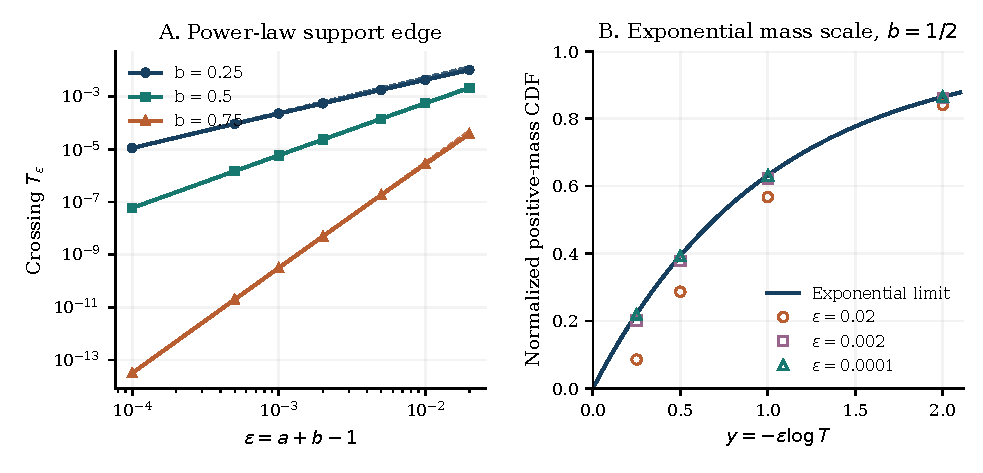
\includegraphics[width=\textwidth]{figures/real_boundary_two_scales.pdf}
\caption{The two scales of endpoint concentration. Left: numerical
crossings (markers) and the leading power laws (dashed curves) at three
fixed inner orders. Right: four sampled distribution-function values
for each indicated $\varepsilon$ at $b=1/2$, compared with the proved
unit-exponential limit. These are diagnostics of the analytic results.}
\label{rwbound:real:fig:boundary}
\end{figure}

All limits in this section keep $b$ fixed. As $b\downarrow0$, the
small parameter $\tau_\varepsilon/\varepsilon$ has exponent
$b/(1-b)\downarrow0$, so the stated hierarchy is not uniform at that
endpoint. As $b\uparrow1$, the exponent $1/(1-b)$ and the constants
become singular. Joint limits involving either endpoint require
additional analysis and are not consequences of these theorems.
